The advances in making sailboat more autonomous open new perspective in a few domains, such as marine research, a boat that can stay at sea more than on day without surveillance and can change location where the user of the boat would want it to go. This is the goal of \r{A}land Sailing Robots a project of \r{A}land University of Applied Science (H\"{o}gskolan p\r{a} \r{A}land), developing a sailboat environment-friendly and usable in research, the project is funded by the European Regional Development Fund.

A research that the boat could do is the survey for harbour porpoises (\textit{Phocoena phocoen})in the Baltic sea as it an endangered species, in the current state there is fixed buoys to detect those animals in certain places,  but they does not cover every places, a autonomous sailboat would open the possibility of easy survey of any area not covered by the buoys without the noise created by a motorized manned boat.

\begin{figure}[H]
\centering
    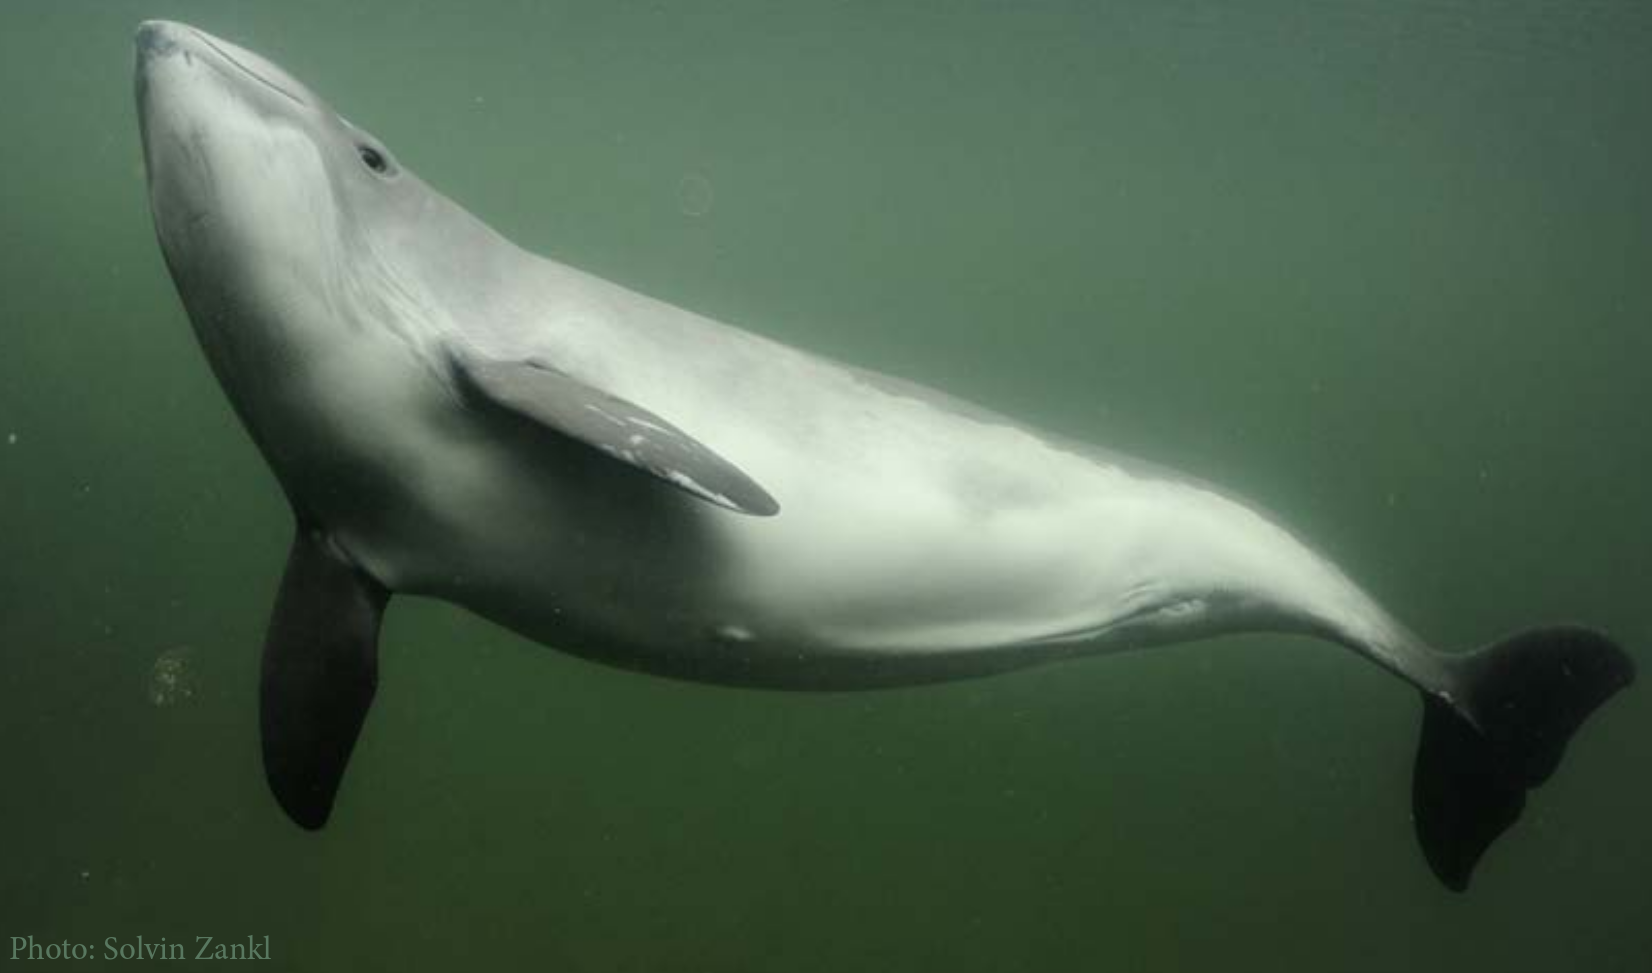
\includegraphics[scale=0.10,angle=0]{porpoise.png}
    \caption{Harbour Porpoise  photo: Solvin Zankl }
    \label{fig:porpoise}
\end{figure}

When using a boat the researcher need to have a cable, an array of hydrophones that will go deep enough to increase the signal-to-noise ratio because the surface of the sea create a lot of noise that would block the detection of the animals , a cable of hydrophones can reach 20 meters.


\begin{figure}[H]
\centering
    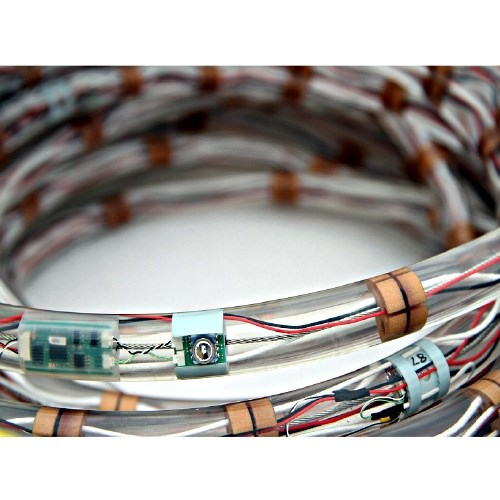
\includegraphics[scale=0.25,angle=0]{array_hydro.jpg}
    \caption{Array of Hydrophones NarcineArray from SEA }
    \label{fig:arrayHydro}
\end{figure}


The main goal of this report is to determine the viability of a small sailboat to carry such a cable. It will be done by simulation and field test. The modelling of a cable can be done with different ways such as finite elements for the more complicated solutions or by assimilating the cable as multiple connected rods. The last method as been chosen for the model. Following the work of~\cite{johansen2007modelling} (the goal was to not be dependent on a particular external software for multi-body dynamics).\\
The cable simulation will be then added to the modified sailboat model to take into account the effect of
the cable on the sailboat and model the behaviour of the boat and the cable.

Then tests have been done with the project sailboat, the result will be compared to the simulation and use to determine the possibilities of the towing sailboat.